\documentclass[12pt,letterpaper]{article}
\usepackage[parfill]{parskip}
\usepackage{graphicx}
\graphicspath{ {./images/} }

\begin{document}

\section*{CptS 453 | Homework-02 }
\subsection*{Charles Nguyen, \#011606177 }

\subsection*{Problem 1:}

The bounds for a \emph{biparte} graph are as follows:

- The lower bound is when the graph is extremely skewed to one side, where
$n_i$ == 1 for either side of the biparte graph and $n_j = 200 - n_i $ is the
remaining side. Thus, the lower bound is $m = 200$.

- The upper bound is when the graph is perfectly symmetrically, where $n_i ==
n_j$. In this case,

\[n_i = n_j = 100 \]

Thus,

\[ m = n_i \cdot n_j \mbox{, where} n_i = n_j \]

\subsection*{Problem 2:}

Similarly, for $p$ and $q$ as integers, where $p < q$. The lower bound of
$K_{p,q}$ is the product $p \cdot q$, where $p == 1$.  The upper bound is $((p
+ q) / 2)^2$.

\pagebreak

\subsection*{Problem 3:}

The set of value $k$ for which $G_k$ is connected is controlled by the
following conditions:

- k where k is prime

- k where $\|j - i\| == k \% 10$

- k where $10 \% k \neq 0$

Since I'm not used to set theory, I am just listing the related subsets. There
should be a relation among these subsets. I am suspecting the following:

\[ \{k \mbox{ is prime}\} \cup (\{\|j-i\| == k\%10\} \cap \{10\%k \neq 0\}) \]

The set of k is $k = \{1, 3, 7\}$.

\pagebreak
\subsection*{Problem 4:}

A cubic graph is a \emph{3-regular} graph, i.e. where all vertices have
\emph{degree} $k=3$.

\subsubsection*{a.}

\emph{Proof:}

A complete graph has every \emph{pair} of distinct vertices connected by a
unique edge. A complete graph is maximally connected, i.e. the number of edges
is maximum and is given by,

\[ {n \choose 2} = \frac{n(n-1)}{2} \]

where $k=n-1$, $n=k+1$.

Thus, it becomes $\frac{nk}{2}$. This quantity has to yield an integer and
therefore $nk$ must be even. Recall that for a cubic graph the degree $k = 3$,
thus $n$ must be an even value.

\subsubsection*{b.}
Given the proof above, in order for a cubic graph of order $n=4$ to exist, we
can see right away that the degree $k=n-1=3$. Thus the number of edges in the
graph will be $\frac{nk}{2} = 6$. The following image shows such a graph:

\begin{figure}[h]
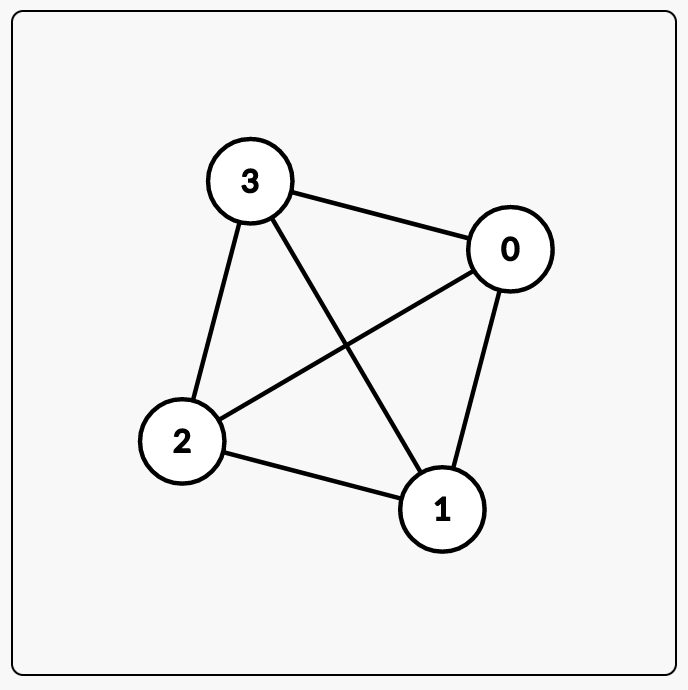
\includegraphics[scale=0.20]{n4k3}
\centering
\end{figure}

\subsubsection*{c.}
Given input $V$ of order $2n$, we can decompose $V$ into $V_1$ of order $n$
and $V_2$ of the same order $n$.  This allows us to construct a \emph{biparte} graph of degree $k=n$.

\end{document}
